\documentclass[11pt,a4paper]{article}
\usepackage[T1]{fontenc}
\usepackage[utf8]{inputenc}
\usepackage{lmodern}
\usepackage[margin=2.2cm]{geometry}
\usepackage{graphicx}
\usepackage{booktabs}
\usepackage{array}
\usepackage{amsmath}
\usepackage{microtype}
\usepackage[font=small,labelfont=bf]{caption}
\usepackage[colorlinks=true,linkcolor=black,citecolor=black,urlcolor=blue]{hyperref}
\usepackage{url}
\setlength{\parskip}{3pt}
\renewcommand{\arraystretch}{1.12}
\newcommand{\ci}[2]{[#1,\,#2]}

\title{Evaluating Retrieval-Augmented Question Answering\\over Indian IPO Offer Documents:\\A Reproducible Ablation Study}
\author{Sarvesh \\ Minor specialization in Big Data Analytics}
\date{}

\begin{document}
\maketitle

\begin{abstract}
Draft Red Herring Prospectuses (DRHPs) and Red Herring Prospectuses (RHPs) are filed with the Securities and Exchange Board of India (SEBI) and routinely run past 500 pages, mixing narrative text with dense financial tables. We build a retrieval-augmented generation (RAG) pipeline for these documents and, more importantly, a reproducible evaluation framework that tests which of its design choices actually matter. The framework combines an evidence-group gold set of 121 questions over 12 filings, retrieval metrics scored at the page level, deterministic grounding checks, a gold-versus-prediction LLM judge, and paired statistics with pre-registered adoption rules. Five single-factor ablations (chunking and parent expansion, table representation, retrieval mode, numeric and citation verification, embedding model) show one clear effect: hybrid retrieval, which fuses dense and BM25 rankings, finds the required pages more often than dense retrieval alone (pooled recall@5 0.578 versus 0.468, McNemar $p=0.015$). The other choices change recall by about $\pm0.05$ or less and none is statistically distinguishable from the baseline. Giving the generator the gold evidence pages raises the judge score from 0.59 to 0.84, so retrieval, not generation, is the main bottleneck, and questions that span two filings are the weakest category. On a 52-question subset of FinanceBench the same pipeline reaches only 0.33 recall@5; the correct filing is identified for 88\% of questions but the page is not, because the evidence is mostly near-identical financial statement tables and many answers are computed from several figures. We release code, gold sets, and per-experiment reports.
\end{abstract}

\section{Introduction}
An investor reading an offer document wants a specific answer, such as the offer size, the registrar, the auditor, or the profit for a fiscal year, together with the page it came from. In Indian IPOs this information is spread over documents of 400 to 700 pages. The documents are long, repetitive (the same figure appears in the summary, the financial statements, and the management discussion), and heavy with tables. A question-answering system for them must find the right pages, quote figures exactly, and decline to answer when the document does not contain the answer; for draft filings this is common, because the final price is printed as a blank.

Retrieval-augmented generation is the standard approach, but the number of design choices is large: how to split a page into chunks, whether to return the surrounding section, how to represent tables, whether to use dense embeddings, keyword search, or both, and whether to verify figures after generation. Most reports justify these choices with a few examples. Our aim is a defensible answer to the question \emph{which of these choices is supported by measurements?}

\paragraph{Research questions.}
\textbf{RQ1:} Which pipeline components improve retrieval and answer quality on Indian IPO documents? \textbf{RQ2:} Where is the bottleneck, in retrieval or in generation? \textbf{RQ3:} Do the findings transfer to a different corpus, namely US SEC filings in the FinanceBench benchmark?

\paragraph{Contributions.}
(1) A config-driven RAG pipeline for SEBI offer documents in which every ablation factor is a field in a configuration object. (2) An evaluation framework with an evidence-group gold set, page-level retrieval metrics, deterministic grounding checks, a gold-versus-prediction judge, paired statistics, and pre-registered adoption rules. (3) Five single-factor ablations on 12 filings with a held-out test split, a ceiling analysis that separates retrieval from generation, and a failure taxonomy. (4) An external check on FinanceBench with a diagnosis of why retrieval is weak there. (5) A small demo application, \emph{Prospectus Desk}, that exposes the answer, its citations, the source page, and the retrieval trace.

\section{Related Work}
\paragraph{Retrieval-augmented generation.}
Lewis et al.\ introduced RAG as retrieval over a document index feeding a generator \cite{lewis2020rag}. Hybrid retrieval, which combines lexical scoring such as BM25 \cite{robertson2009bm25} with dense embeddings, is commonly fused by reciprocal rank fusion \cite{cormack2009rrf}. Cross-encoder rerankers refine a candidate list \cite{nogueira2019rerank}, and the position of evidence in the prompt matters, with models using information at the start and end of a context better than in the middle \cite{liu2023lost}. We use the BGE and E5 embedding families \cite{xiao2023bge,wang2022e5}.

\paragraph{Evaluating RAG.}
RAGAS defines reference-free metrics for faithfulness, answer relevance and context relevance \cite{es2023ragas}; ARES trains lightweight judges for the same dimensions \cite{saadfalcon2023ares}; RAGChecker evaluates at the claim level \cite{ru2024ragchecker}. LLM judges are convenient but carry known biases \cite{zheng2023judge}. Reference-free metrics need no gold answers, but they cannot say whether the \emph{right} page was retrieved. We therefore score retrieval against annotated evidence pages and judge answers against a reference answer, and we add deterministic checks that do not depend on a judge.

\paragraph{Financial document QA.}
FinanceBench is a benchmark of questions over US 10-K, 10-Q and earnings filings, and shows that retrieval over a shared index across companies is far harder than over the right document \cite{islam2023financebench}. Studies of chunking for financial reports find that element-based chunking helps retrieval and question answering \cite{yepes2024chunking}. To our knowledge there is no comparable benchmark for Indian IPO offer documents, which is the gap this work addresses.

\section{System}
\begin{figure}[t]
\centering
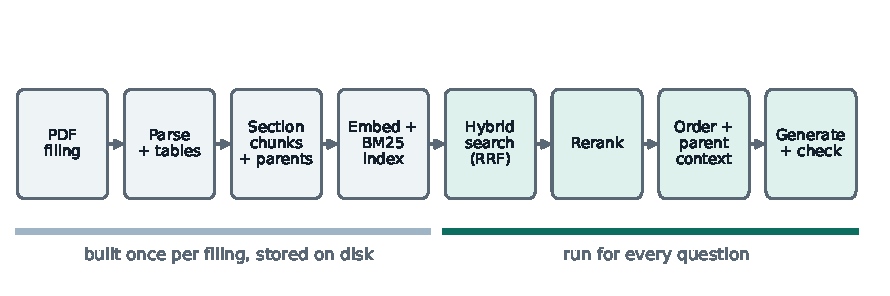
\includegraphics[width=\textwidth]{figs/pipeline.pdf}
\caption{The pipeline. Indexing runs once per filing and is stored on disk; the remaining stages run for every question. Every stage is a field in a configuration object, which is what makes single-factor ablations possible.}
\label{fig:pipeline}
\end{figure}

\subsection{Corpus and parsing}
The corpus has 12 filings (3 RHPs/prospectuses and 9 DRHPs) from Zomato, Nykaa, Swiggy, LIC, Ola Electric, Hyundai Motor India, HDB Financial Services, LG Electronics India, Delhivery, Manipal Health, Jio Platforms and NSE, 6{,}718 pages in total (Table~\ref{tab:corpus}). Text is extracted with PyMuPDF in reading order. Tables are detected with the PyMuPDF table finder and cached, because detection takes minutes per filing. Chapter boundaries (``Risk Factors'', ``Our Business'', ``Management's Discussion and Analysis'', and so on) are detected from page headings and used for chunk boundaries.

\begin{table}[t]
\centering
\caption{Filings and the document-level split. Dev is used for every design decision, test is used once at the end.}
\label{tab:corpus}
\small
\begin{tabular}{llr|llr}
\toprule
Dev filing & Type & Pages & Test filing & Type & Pages \\
\midrule
Zomato & RHP & 420 & Nykaa & RHP & 601 \\
LIC & DRHP & 652 & Swiggy & RHP & 541 \\
Ola Electric & DRHP & 444 & Hyundai Motor India & DRHP & 436 \\
Delhivery & DRHP & 581 & HDB Financial & DRHP & 713 \\
Manipal Health & DRHP & 732 & LG Electronics India & DRHP & 456 \\
 & & & Jio Platforms & DRHP & 528 \\
 & & & NSE & DRHP & 614 \\
\bottomrule
\end{tabular}
\end{table}

\subsection{Chunking and hierarchy}
The baseline splits each chapter into paragraph-packed child chunks of about 1{,}000 characters with 150 characters of overlap, and groups consecutive children of the same chapter into parent blocks of about 3{,}000 characters. Children are embedded and searched. When a child is selected, its parent is returned as context if it is shorter than 4{,}000 characters, otherwise the child itself is used. This gives precise matching with enough surrounding text for the generator. Tables are indexed as separate chunks.

\subsection{Retrieval}
Each question is embedded with \texttt{bge-small-en} (384 dimensions) and compared by exact cosine similarity with all chunk embeddings of the selected filings; a vector database is unnecessary because a filing holds a few thousand chunks, and exact search avoids approximate-search recall as a confounder. In parallel, BM25 scores the same chunks. The two rankings are fused with reciprocal rank fusion (equal weights, $k=60$), the top 10 candidates are reranked with a cross-encoder (\texttt{ms-marco-MiniLM-L-6-v2}), and the top 5 are kept. Retrieved context is ordered to place the strongest passages at the start and end of the prompt, following \cite{liu2023lost}. Retrieval is run over the open corpus of all 12 filings with no document router, so the system must also pick the right company from the question.

\subsection{Generation and verification}
The generator is prompted to answer only from the supplied context, cite every claim as \texttt{[Company, Page: N]}, and reply with a fixed sentence when the context does not contain the answer. With \emph{verification} on, every number in the answer must appear in the retrieved text and every cited page must be among the retrieved pages. On failure the model is asked once to rewrite the answer using only supported figures; if figures remain unsupported, the system abstains.

\section{Evaluation Framework}
\subsection{Gold set}
The gold set (\texttt{gold\_v1}) has 121 questions: 53 on the five dev filings and 68 on the seven test filings (Table~\ref{tab:gold}). Questions were drafted by an LLM from sampled pages, then filtered automatically (the supporting quote must occur on the source page, the question must be self-contained and name the company, and it must not copy more than five consecutive words from the page) and verified by a second LLM. Evidence was then expanded: every other page that states the same quote, number, or a close lexical match was judged by the verifier and added to the question's evidence if it supports the answer. Evidence is stored as \emph{groups}: a question needs at least one page from every group. The set also contains multi-document questions that need two filings, and unanswerable questions (for instance, the final offer price of a draft filing, or a revenue figure for a future year). The project author audited the set; all numbers in this report are computed against this audited version.

\begin{table}[t]
\centering
\caption{Gold-set composition (\texttt{gold\_v1}). Retrieval metrics are computed on answerable questions only: 48 dev and 61 test.}
\label{tab:gold}
\small
\begin{tabular}{lrrrrrrrr}
\toprule
 & Factoid & Numeric & Table & List & Definition & Two filings & Unanswerable & Total \\
\midrule
Dev & 10 & 10 & 10 & 10 & 3 & 5 & 5 & 53 \\
Test & 13 & 13 & 14 & 11 & 3 & 7 & 7 & 68 \\
\midrule
Both & 23 & 23 & 24 & 21 & 6 & 12 & 12 & 121 \\
\bottomrule
\end{tabular}
\end{table}

\subsection{Metrics}
\paragraph{Retrieval.} For each question we compute hit, full-hit, recall, precision, MRR and nDCG at the page level, at three points: the fused candidates before reranking (\texttt{cand}), the final top five (\texttt{final}), and the assembled context (\texttt{ctx}). Recall is the share of evidence groups covered; full-hit requires all of them.

\paragraph{Grounding (no LLM).} Key-fact recall (are the gold key values present in the answer?), numeric support and unsupported figures (does every figure in the answer appear in the retrieved text? page numbers inside citations, including ranges, are excluded), citation validity (are cited pages among the retrieved ones?), and abstention: false abstention on answerable questions and correct abstention on unanswerable ones.

\paragraph{Answer quality (LLM judge).} The judge sees only the question, the gold answer and the predicted answer. It splits the gold answer into items and grades three axes on five levels (excellent, good, acceptable, bad, extremely bad, mapped to 1.0, 0.75, 0.5, 0.25, 0): \emph{coverage} (are all gold items present?), \emph{faithfulness} (are the predicted items accurate relative to the gold answer, with none invented?), and \emph{redundancy} (is each item stated once?). The overall score is their mean, and an abstention on an answerable question scores 0 without a judge call. We use a single judge, \texttt{gpt-oss-120b}. On 83 dev answers, the judge's coverage agrees with the deterministic key-fact check on 84\% of answers (Pearson $r=0.56$).

\subsection{Statistics and pre-registration}
Differences between configurations are paired by question. We report bootstrap 95\% intervals on per-question differences and exact McNemar tests on binary hit outcomes, with Holm correction within a study. Adoption rules were fixed before the test split was touched: a non-baseline level replaces the baseline only if its improvement is supported (interval above zero, or Holm $p<0.05$ in its favour); verification is adopted only if it reduces unsupported figures without lowering the judge score by more than 0.03; and the generator is the one with the highest mean judge score on dev among those with a failure rate of at most 10\% (ties go to the cheaper model). Decisions are made on dev and confirmed on test; a pooled dev-plus-test analysis adds power but does not change decisions.

\section{Experimental Setup}
Table~\ref{tab:ablations} lists the five single-factor studies. In each study one factor varies and everything else stays at the baseline (marked with an asterisk in the table). Held fixed throughout: equal RRF weights, the MiniLM reranker, context ordering, the parent-size cap, and no query rewriting. Three generators were compared on the NVIDIA-hosted Nemotron family: \texttt{bolt} (4B-class, fast, used for ablations), \texttt{nano} (30B reasoning model) and \texttt{ultra} (550B). The rule above selected \texttt{nano} on dev (Section~\ref{sec:gen}).

\begin{table}[t]
\centering
\caption{The five ablation studies. The baseline level is marked with an asterisk.}
\label{tab:ablations}
\small
\begin{tabular}{@{}p{3.6cm}p{4.2cm}p{6.6cm}@{}}
\toprule
Study & Levels & What varies \\
\midrule
1 Chunking and hierarchy & fixed, section, section+parent*, section+parent+header & Chunk boundaries; whether the parent section is returned; whether the chapter name is prepended to a chunk \\
2 Table representation & inline, flat, markdown* & How a detected table is written into text \\
3 Retrieval mode & dense, BM25, hybrid* & Embedding search, keyword search, or both fused by RRF \\
4 Verification & off*, on & Check figures and citations against the retrieved text, rewrite once, else abstain \\
5 Embedder & bge-small*, bge-large, e5-large & Embedding model (study run on one filing set at a time for compute) \\
\bottomrule
\end{tabular}
\end{table}

A note on a bug found by the evaluation itself: the initial hybrid configuration inherited RRF weights of 0.6 and 0.4, with which keyword-only hits could never enter the candidate cut-off, so ``hybrid'' retrieval was identical to dense retrieval. The ablation showed the two as identical to the digit, which exposed the problem; the weights were set to the standard equal weighting and a regression test was added. A second bug counted the second page in a citation range such as ``Page: 266--267'' as an unsupported figure and flagged about half of all answers; it was fixed and all generation runs repeated.

\section{Results}
\subsection{Retrieval ablations}
Hybrid retrieval is the only change with a clear effect (Figure~\ref{fig:mode}). On dev, hybrid reaches recall@5 of 0.635 against 0.469 for dense retrieval (difference $-0.167$, McNemar $p=0.016$; dense found a required page that hybrid missed on no question, and missed one that hybrid found on eight). On test the gap is smaller and not significant on its own (0.533 versus 0.467), but pooled over 109 questions it is $-0.110$ with interval \ci{-0.18}{-0.04} and $p=0.015$. BM25 alone is competitive: it is lower than hybrid on dev (0.573), higher on test (0.582), and equal pooled (0.578). Hybrid is therefore preferable to dense retrieval, and not demonstrably better than keyword search.

\begin{figure}[t]
\centering
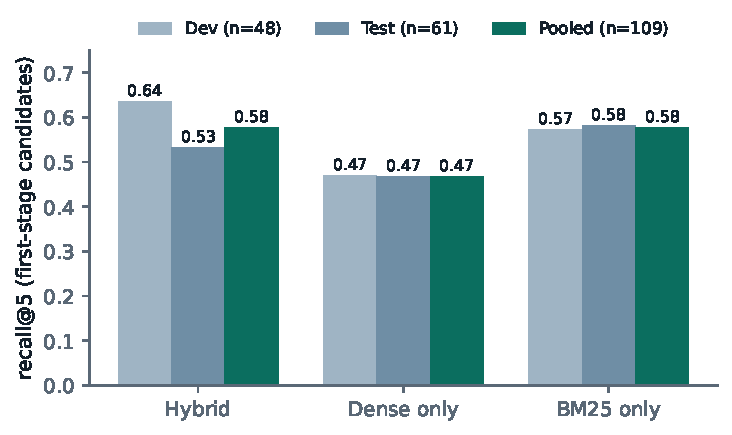
\includegraphics[width=0.7\textwidth]{figs/retrieval_mode.pdf}
\caption{Retrieval mode: recall@5 of the first-stage candidates. Hybrid beats dense retrieval pooled over dev and test ($p=0.015$); BM25 matches hybrid.}
\label{fig:mode}
\end{figure}

None of the other factors is distinguishable from the baseline (Figure~\ref{fig:forest}, Table~\ref{tab:retr}). Fixed windows, flat chunks, and the chapter-name header move final recall@5 by at most $0.05$ on either split. Inline table text is lowest on dev (0.573 versus 0.635 for markdown, $p=0.5$) but ties on test (0.656), and on the 20 dev questions that need a table or figure it gives 0.700 against 0.800. Larger embedding models give $+0.021$ (bge-large) and $0.000$ (e5-large) on dev and $+0.008$ and $+0.033$ on test, none significant, at roughly eight times the indexing cost. The parent block does not change which pages are retrieved (flat and parent variants have identical recall by construction); its effect is on the generator, shown next.

\begin{figure}[t]
\centering
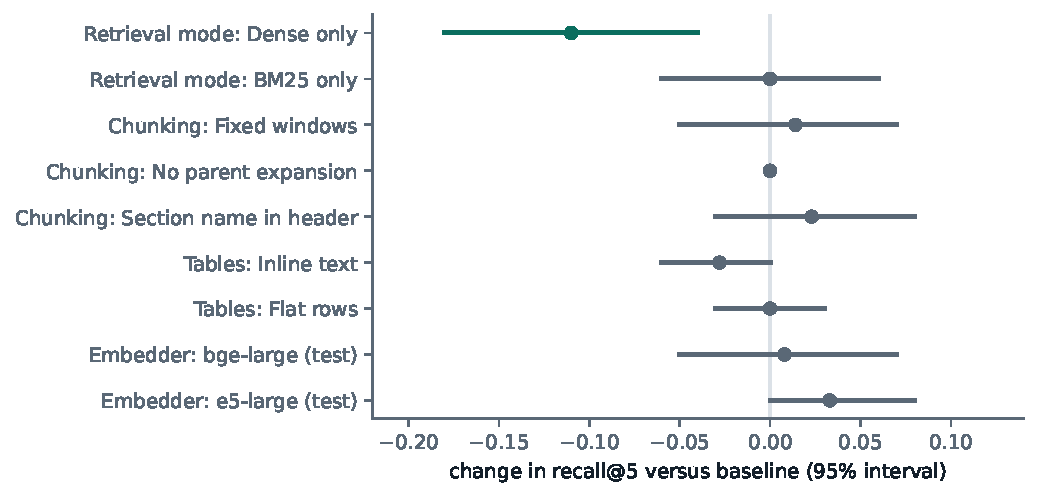
\includegraphics[width=0.72\textwidth]{figs/forest.pdf}
\caption{Change in recall@5 relative to each study's baseline, pooled over dev and test (embedder rows: test split). Bars are 95\% intervals. Only dense-only retrieval excludes zero.}
\label{fig:forest}
\end{figure}

\begin{table}[t]
\centering
\caption{Final recall@5 for the retrieval studies. The baseline is the first row of each block. The embedder study is evaluated on the filing set of each split.}
\label{tab:retr}
\small
\begin{tabular}{llrr}
\toprule
Study & Level & Dev (n=48) & Test (n=61) \\
\midrule
Chunking & section+parent (baseline) & 0.635 & 0.656 \\
 & fixed, flat & 0.625 & 0.689 \\
 & section, flat & 0.635 & 0.656 \\
 & section+parent+header & 0.625 & 0.705 \\
\midrule
Tables & markdown (baseline) & 0.635 & 0.656 \\
 & inline & 0.573 & 0.656 \\
 & flat & 0.656 & 0.639 \\
\midrule
Embedder & bge-small (baseline) & 0.698 & 0.672 \\
 & bge-large & 0.719 & 0.680 \\
 & e5-large & 0.698 & 0.705 \\
\bottomrule
\end{tabular}
\end{table}

\subsection{Answer-level studies}
Verification lowers the share of answers containing a figure absent from the retrieved text, from 5.8\% to 1.9\% pooled over dev and test (nano generator), and leaves the judge score essentially unchanged (0.622 to 0.636, difference $+0.005$ with interval \ci{-0.02}{0.04}). False abstention is also unchanged (0.283 versus 0.276). Unsupported figures were already rare with the verified prompt, so the check removes a small number of errors without costing quality.

Removing parent expansion lowers answer quality for both generators on dev and test, though only the bolt effect is clearly outside noise: pooled judge score falls from 0.622 to 0.595 for nano (interval \ci{-0.07}{0.03}) and from 0.589 to 0.496 for bolt (difference $-0.093$, interval \ci{-0.15}{-0.05}). The smaller generator profits more from the extra section text, a plausible effect that we did not test further.

\subsection{Generator selection}\label{sec:gen}
Table~\ref{tab:gen} compares the three generators with the baseline pipeline. On dev, nano has the highest judge score (0.594 against 0.580 for bolt and 0.566 for ultra) and the selection rule picks it; the three are statistically indistinguishable. On test, ultra is nominally highest (0.650 against 0.643 for nano), again within noise, and about twice as slow as nano at the median. We keep the pre-registered choice and report the test ordering as it came out rather than reselecting.

\begin{table}[t]
\centering
\caption{Generator comparison with the baseline pipeline. Overall is the mean judge score; latency is the median generation time.}
\label{tab:gen}
\small
\begin{tabular}{llrrrrr}
\toprule
Split & Generator & Overall & Faithfulness & Fail rate & False abst. & p50 s \\
\midrule
Dev (n=53) & bolt & 0.580 & 0.750 & 0\% & 0.312 & 1.05 \\
 & nano & 0.594 & 0.758 & 4\% & 0.304 & 4.83 \\
 & ultra & 0.566 & 0.800 & 0\% & 0.375 & 8.54 \\
\midrule
Test (n=68) & bolt & 0.597 & 0.835 & 0\% & 0.328 & 1.87 \\
 & nano & 0.643 & 0.812 & 1\% & 0.267 & 3.36 \\
 & ultra & 0.650 & 0.884 & 0\% & 0.295 & 6.48 \\
\bottomrule
\end{tabular}
\end{table}

\subsection{Retrieval versus generation}
To separate the two stages we gave the generator the gold evidence pages instead of the retrieved ones (a ceiling run). On dev, nano's judge score rises from 0.59 to 0.84, a retrieval loss of $+0.27$ with interval \ci{0.10}{0.43}; bolt rises from 0.58 to 0.79 ($+0.21$, interval \ci{0.04}{0.38}), see Figure~\ref{fig:ceiling}. The largest losses are on multi-document questions (nano 0.20 to 0.60; bolt 0.00 to 0.75) and numeric questions (nano 0.56 to 0.93). Retrieval is therefore the main source of error, and improving the generator can recover at most part of the gap.

\begin{figure}[t]
\centering
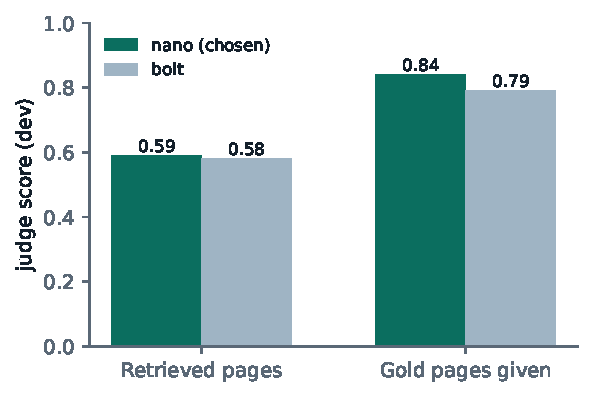
\includegraphics[width=0.5\textwidth]{figs/ceiling.pdf}
\caption{Judge score on dev with retrieved pages versus gold pages given to the generator.}
\label{fig:ceiling}
\end{figure}

\subsection{Final test run and failure analysis}
With the baseline configuration (no component replaced, generator nano), the one-shot test run on 68 questions gives recall@5 of 0.656 \ci{0.54}{0.77}, nDCG@5 0.534, judge overall 0.651, coverage 0.621, faithfulness 0.824, key-fact recall 0.580, unsupported figures in 7.4\% of answers, false abstention 26.7\%, and correct abstention on all seven unanswerable questions. When each question is limited to its own filing (oracle retrieval), recall@5 rises to 0.787 \ci{0.68}{0.89}, which shows that choosing the right company accounts for about 0.13 of recall.

Performance depends strongly on the question type (Figure~\ref{fig:type}). Table questions are solved (recall 1.00, judge 0.89), factoid and list questions are good (recall 0.77 and 0.73), numeric questions are mediocre (0.46) and questions spanning two filings fail (0.14 recall, judge 0.29). Sorting each test answer by outcome (Figure~\ref{fig:tax}) shows that 41 of 68 are right (34 good answers and 7 correct abstentions), 20 fail because the evidence was not retrieved (14 abstained, 6 answered without it), and only 7 fail with the evidence in hand (4 poor answers, 2 abstentions despite evidence, 1 failed generation). Most failures thus start in retrieval.

\begin{figure}[t]
\centering
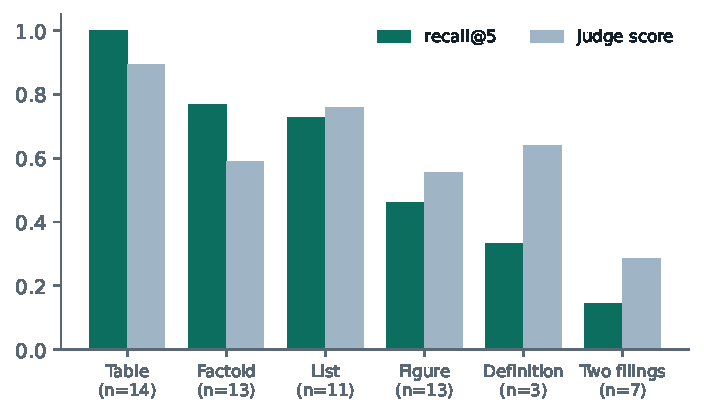
\includegraphics[width=0.7\textwidth]{figs/by_type.pdf}
\caption{Final test run by question type. Table questions are solved; two-filing questions are not.}
\label{fig:type}
\end{figure}

\begin{figure}[t]
\centering
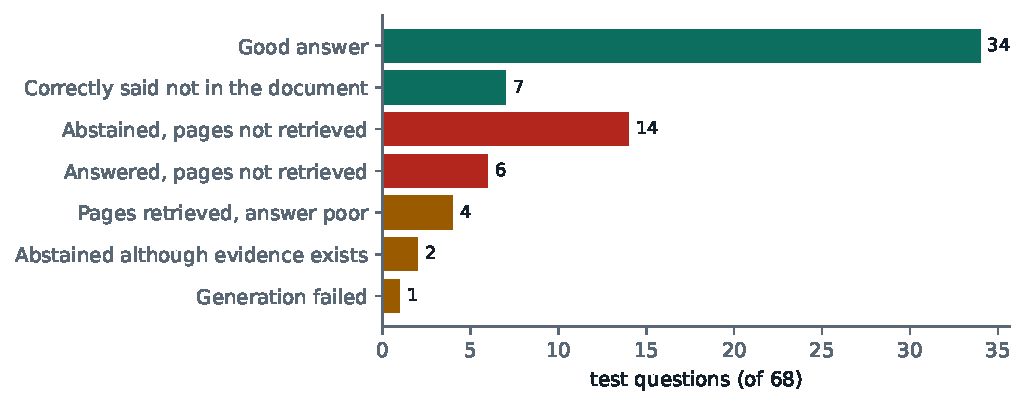
\includegraphics[width=0.7\textwidth]{figs/taxonomy.pdf}
\caption{Outcome of each of the 68 test questions.}
\label{fig:tax}
\end{figure}

\section{External Validity: FinanceBench}
\subsection{Setup}
We selected 52 questions from the 150-question open FinanceBench set that refer to 12 filings (nine 10-Ks, two 10-Qs and one earnings release, 3M, AES, Amcor, AMD, American Express, Best Buy, Boeing, CVS Health, PepsiCo and Ulta Beauty) and indexed all 12 together, so the open-corpus setting matches the IPO experiments. Evidence pages come from the benchmark annotations; questions that need several pages count as several evidence groups. Nothing in the pipeline was tuned for these filings. We also tried a US layout labeler (detecting ``Item 1A'', ``Item 7'' and the primary financial statements) in place of SEBI chapter detection.

\subsection{Results}
Final recall@5 is 0.333 \ci{0.21}{0.47} for the baseline, 0.314 for dense retrieval, and 0.179 for BM25. Unlike on IPO documents, hybrid and dense retrieval tie (differences within $\pm0.03$) and BM25 is significantly worse (cand.recall 0.122 against 0.276, $p=0.043$); the variants of chunking and table handling differ by less than 0.07 (Figure~\ref{fig:fb}). The US layout labels change nothing: baseline recall stays at 0.333, and the oracle setting moves from 0.401 to 0.420. Adding the section name to the chunk header lifts first-stage recall from 0.276 to 0.346 but the cross-encoder reranker then lowers final recall to 0.269, so the label helps the first stage and the reranker undoes it. With nano, the judge score is 0.344, and with the gold pages given it is 0.594; verification does not help (0.344 to 0.310, not significant).

\begin{figure}[t]
\centering
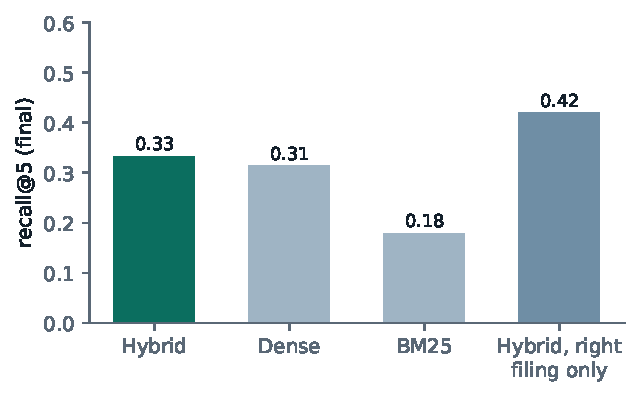
\includegraphics[width=0.55\textwidth]{figs/financebench.pdf}
\caption{FinanceBench subset (52 questions): final recall@5 by retrieval mode, and with search restricted to the right filing.}
\label{fig:fb}
\end{figure}

\subsection{Why retrieval is weak}
A breakdown of the baseline run points to five causes.
\begin{enumerate}
\item \textbf{The filing is found; the page is not.} The right filing appears in the top five for 88\% of questions, and restricting search to it lifts recall only to 0.42. Confusion between filings is not the main cause, although 10 of 52 questions retrieve a page from a sibling 10-K or 10-Q of the same company.
\item \textbf{Multi-page evidence.} The 43 questions with one evidence page reach 0.395 recall; the nine with two or three pages reach 0.00 and 0.11, because every evidence group must be hit.
\item \textbf{Look-alike statement tables.} Of the 66 annotated pages, 27 are income statement, balance sheet or cash flow pages and 10 are notes tables. Their text is dominated by shared line-item names and numbers, so both embeddings and BM25 return many similar pages across companies and years.
\item \textbf{Computed answers.} Only 22 of the 39 questions with numeric key facts have all of them verbatim on the annotated pages; the rest are ratios or derived values whose inputs sit on pages that do not resemble the question (for example, whether a company is capital intensive).
\item \textbf{Page-level scoring is strict.} For the 22 extractive questions the answer figures occur in the retrieved top five for 18 of them, including 9 of the 13 counted as misses. Short figures can match by chance, so this is an upper bound, but it shows that other valid pages exist. Only 5 of 35 missed questions retrieved a page within two pages of an annotated page.
\end{enumerate}

\subsection{Comparison with published pipelines}
Published FinanceBench numbers report answer accuracy on the 150-question set, which differs from our page recall and judge score in subset, metric and grader, so they give context and not a head-to-head comparison. The benchmark paper reports GPT-4-Turbo with a shared vector store over all filings at 19\% correct (68\% refused), against 50\% with a per-document store \cite{islam2023financebench}; a vendor re-run reports 27\% for a shared store at top-8 and 51\% for a single store at top-32 \cite{ragie2024}. The same pattern appears here: searching all filings together is far worse than searching the right one, with recall 0.33 against 0.42 in our oracle setting, and the judge score with gold pages (0.59) is far higher than with retrieved pages (0.34). We did not run those systems ourselves.

\section{Demonstration}
Prospectus Desk (Figure~\ref{fig:demo}) is a small web application over the same pipeline. A user selects filings, asks a question, and sees the answer with page citations as buttons that open the source page with the answer's figures highlighted. Beside the answer, a trace shows the dense, keyword, fused and reranked lists, with the reference-set evidence marked for example questions. A compare view runs two settings on the same question (hybrid versus dense, figure check on or off, with or without surrounding text), and a results view charts the findings of this report. The six built-in examples come from the test split and include failures on purpose; answers are cached so the demo works without an API connection.

\begin{figure}[t]
\centering
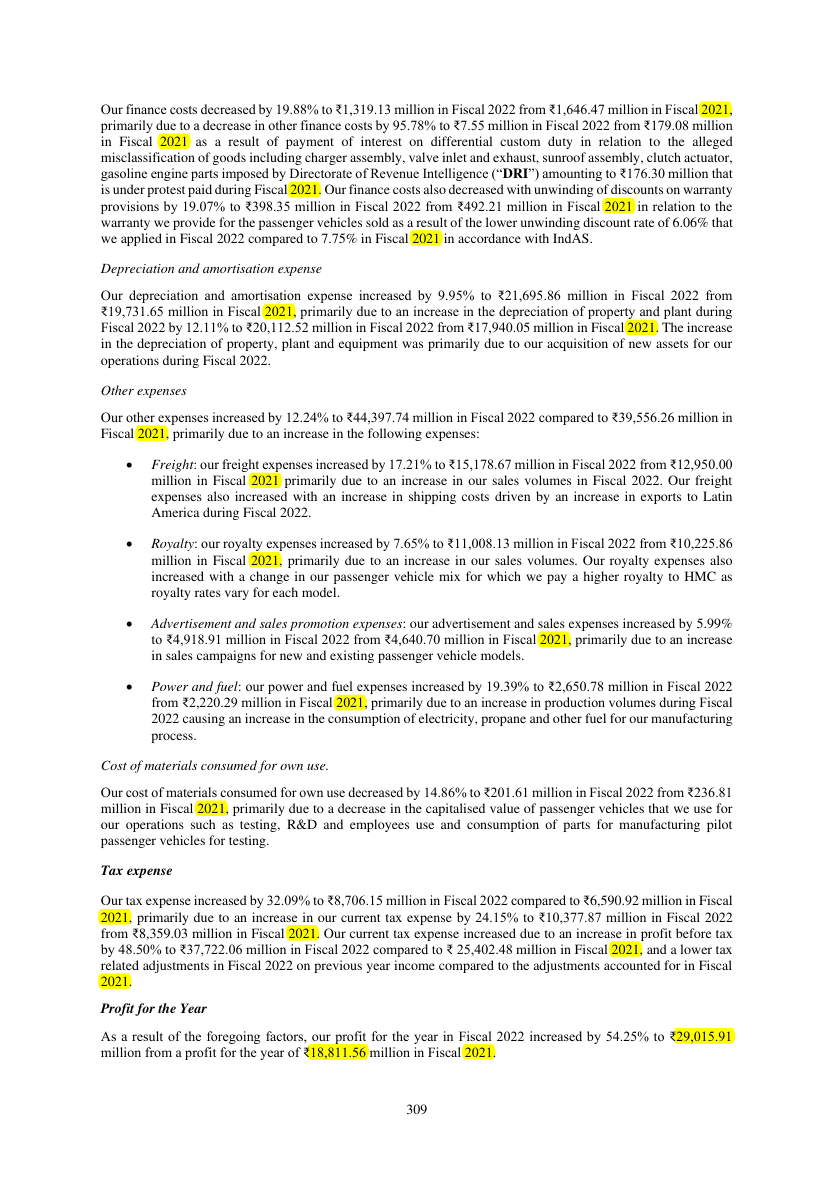
\includegraphics[width=0.46\textwidth]{figs/demo_page.png}
\caption{The source-page viewer in Prospectus Desk: the page cited in an answer (Hyundai Motor India, page 314) with the figures of the answer highlighted, so a reader can check the answer in one click.}
\label{fig:demo}
\end{figure}

\section{Limitations}
\begin{itemize}
\item \textbf{Gold set.} It is LLM-generated, filtered, LLM-verified and then audited by the author; no independent annotator checked it and no inter-annotator agreement was measured. The set is small (48 and 61 answerable questions per split), so intervals are wide (about $\pm0.12$ on recall), and the null results mean ``no effect large enough to detect'', not ``no effect''.
\item \textbf{Single judge.} All judge scores come from one model (\texttt{gpt-oss-120b}), checked against a deterministic metric but not against human grading, and the judge and generators were not independent of the dataset's LLM-built construction.
\item \textbf{Generator choice.} The nano-versus-ultra ordering differs between dev and test; we followed the pre-registered rule, but the differences are within noise.
\item \textbf{Scope.} Twelve filings from one regulator; the embedder study was run on one split's filings at a time; query rewriting, a document router, and learned rerankers were held fixed.
\item \textbf{FinanceBench.} A 52-question subset of 12 filings, scored by page recall, so it cannot be compared directly with published accuracy figures; we did not run external systems.
\item \textbf{Provider and rate limits.} Judging used free-tier quotas, so test-split confirmations were judged in a later pass; results are cached and reproducible, but the hosted models can change.
\end{itemize}

\section{Future Work}
(i) Independent human annotation of a random sample of the gold set and of the judge's outputs, with agreement statistics. (ii) Retrieval for financial statement tables: table-aware indexing that keeps row and column headers with each number, query rewriting for computed questions, and a reranker trained on financial text (on FinanceBench the generic reranker undid a gain from section labels). (iii) Multi-hop or agentic retrieval for questions spanning several filings, the weakest category here. (iv) A document router so that company identification is explicit. (v) Reference-free metrics such as RAGAS as a supplementary row, and a comparison with published FinanceBench systems on the full 150 questions. (vi) A larger corpus and gold set, including final prospectuses that contain the offer price.

\section{Conclusion}
Three findings stand out. First, among five common design choices, only hybrid retrieval has a measurable effect on Indian IPO documents; chunking, table representation, embedding size and verification are within noise and cost little to leave at their defaults. Second, retrieval, not generation, limits answer quality: with the right pages the judge score rises from 0.59 to 0.84, and questions that span two filings fail almost entirely. Third, the findings are partly dataset-specific: on US filings hybrid retrieval does not beat dense retrieval, and weak page-level recall comes from look-alike financial tables and computed answers. The main product of this work is the evaluation framework, which found two bugs in our own pipeline, tested every component against a baseline, and made it clear where to invest next.

\begin{thebibliography}{99}
\small
\bibitem{lewis2020rag} P.~Lewis et al. Retrieval-augmented generation for knowledge-intensive NLP tasks. \emph{NeurIPS}, 2020.
\bibitem{robertson2009bm25} S.~Robertson and H.~Zaragoza. The probabilistic relevance framework: BM25 and beyond. \emph{Foundations and Trends in Information Retrieval}, 3(4):333--389, 2009.
\bibitem{cormack2009rrf} G.~V. Cormack, C.~L.~A. Clarke and S.~Buettcher. Reciprocal rank fusion outperforms Condorcet and individual rank learning methods. \emph{SIGIR}, 2009.
\bibitem{nogueira2019rerank} R.~Nogueira and K.~Cho. Passage re-ranking with BERT. \emph{arXiv:1901.04085}, 2019.
\bibitem{liu2023lost} N.~F. Liu et al. Lost in the middle: how language models use long contexts. \emph{TACL}, 2024 (arXiv:2307.03172).
\bibitem{xiao2023bge} S.~Xiao et al. C-Pack: packaged resources to advance general Chinese embedding (BGE). \emph{arXiv:2309.07597}, 2023.
\bibitem{wang2022e5} L.~Wang et al. Text embeddings by weakly-supervised contrastive pre-training (E5). \emph{arXiv:2212.03533}, 2022.
\bibitem{es2023ragas} S.~Es et al. RAGAS: automated evaluation of retrieval augmented generation. \emph{arXiv:2309.15217}, 2023.
\bibitem{saadfalcon2023ares} J.~Saad-Falcon et al. ARES: an automated evaluation framework for retrieval-augmented generation systems. \emph{arXiv:2311.09476}, 2023.
\bibitem{ru2024ragchecker} D.~Ru et al. RAGChecker: a fine-grained framework for diagnosing retrieval-augmented generation. \emph{arXiv:2408.08067}, 2024.
\bibitem{zheng2023judge} L.~Zheng et al. Judging LLM-as-a-judge with MT-Bench and Chatbot Arena. \emph{NeurIPS Datasets and Benchmarks}, 2023.
\bibitem{islam2023financebench} P.~Islam et al. FinanceBench: a new benchmark for financial question answering. \emph{arXiv:2311.11944}, 2023.
\bibitem{yepes2024chunking} A.~J. Yepes et al. Financial report chunking for effective retrieval augmented generation. \emph{arXiv:2402.05131}, 2024.
\bibitem{ragie2024} Ragie. How Ragie outperformed the FinanceBench test. Company blog post, \url{https://www.ragie.ai/blog/ragie-outperformed-financebench}, accessed 2026.
\end{thebibliography}

\end{document}
